 \makeatletter
\renewcommand{\cleardoublepage}{\clearpage} % Evita páginas en blanco extra
\makeatother

\frontmatter % Use roman page numbering style (i, ii, iii, iv...) for the pre-content pages

\pagestyle{plain} % Default to the plain heading style until the thesis style is called for the body content

%----------------------------------------------------------------------------------------
%	TITLE PAGE
%----------------------------------------------------------------------------------------


\begin{titlepage}
  \begin{center}
  
    % LOGO ARRIBA
    % Ajusta la ruta y el tamaño de tu logo (o quítalo si no quieres poner imagen)
			$if(thesis.logo)$
			$if(thesis.logo-height)$
			\includegraphics[height=$thesis.logo-height$]{$thesis.logo$} % University/department logo
			$else$
			\includegraphics{$thesis.logo$}
			$endif$
			$endif$\\[0.3cm]
    %
\includegraphics[width=2cm]{images/ufpe-logo.png}\\[0.3cm]
    
    % NOMBRES DE LA UNIVERSIDAD/PROGRAMA EN MAYÚSCULAS
    {\large\MakeUppercase{UNIVERSIDADE FEDERAL DE PERNAMBUCO}}\\
    {\large\MakeUppercase{CENTRO DE CIÊNCIAS EXATAS E DA NATUREZA}}\\
    {\large\MakeUppercase{PROGRAMA DE PÓS-GRADUAÇÃO EM ESTATÍSTICA}}\\
    {\large\MakeUppercase{DOUTORADO EM ESTATÍSTICA}}\\[4cm]
		
    % NOMBRE DE LA TESISTA
    {\large ROSA JANETH ALPALA}\\[3cm]
    
    % TÍTULO 
    {\Large \textbf{Entropy-Based Test Statistics for Heterogeneity Detection in SAR Data}}\\[6cm]
    %\textbf{AND CAUSE-SPECIFIC MORTALITY IN ENGLAND}}\\[5cm]
    

		
		%{\Large Doctoral Thesis}\\[2cm] % Thesis type
%
    % CIUDAD Y AÑO
   {\large Recife}\\
   {\large 2025}
    
  \end{center}
\end{titlepage}

\begin{titlepage}
  \thispagestyle{empty}
    \begin{center}
    {\large ROSA JANETH ALPALA}\\[4cm]
    {\Large \textbf{Entropy-Based Test Statistics for Heterogeneity Detection in SAR Data }}\\[4cm]
  \end{center}

  % Quita el \hfill y en lugar de eso usamos \begin{center}...
  %\begin{center}
  \noindent
  \hspace*{0.3\textwidth}
  \begin{minipage}{0.65\textwidth}
    Thesis submitted to the Graduate Program in Statistics at 
    the Universidade Federal de Pernambuco, as a partial requirement 
    for the degree of Doctor of Philosophy  in Statistics.
    
    \vspace{1em}
    \textbf{Concentration area}: Applied Statistics
    
    \vspace{2em} 
    \textbf{Advisor}: Prof. Dr. Alejandro C. Frery \\
    \textbf{Co-advisor}: Prof. Dr. Abraão D. C. do Nascimento
  \end{minipage}
  %\end{center}
  
  \vfill
  \begin{center}
    Recife\\
    2025
  \end{center}
\end{titlepage}

% --- SUBPORTADA O FOLHA DE ROSTO ---

% \begin{titlepage}
%   \thispagestyle{empty} % Quita numeración en esta página
%   
%   \begin{center}
%     % --- NOMBRE DEL ESTUDIANTE --- 
%     {\large ROSA JANETH ALPALA}\\[3cm]
%     
%     % --- TÍTULO EN MAYÚSCULAS O NEGRITA --- 
%     {\Large \textbf{TEST STATISTICS BASED ON ENTROPY FOR HETEROGENEITY DETECTION IN SAR DATA }}\\[3cm]
%     %\textbf{}}\\[3cm]
%   \end{center}
% %Test Statistics Based on Entropy and the Coefficient of Variation for Heterogeneity Detection in SAR Data
%   \hfill
%   \begin{minipage}{0.6\textwidth}
%     % -- TEXTO DESCRIPTIVO --
%     Thesis submitted to the Graduate Program in Statistics of the Universidade Federal de Pernambuco, as a partial requirement for the degree of Doctor in Statistics.
%     
%     \vspace{1em}
%     \textbf{Concentration area}: Applied Statistics
%     
%     \vspace{2em} 
% 		\textbf{Advisor}: Prof. Alejandro C. Frery \\
% 		\textbf{Co-advisor}: Prof. Abraão David Costa do Nascimento
%    
%   \end{minipage}
%   
%   \vfill
%   \begin{center}
%     Recife\\
%     2025
%   \end{center}
% 
% \end{titlepage}

%----------------------------------------------------------------------------------------
%	Actas
%----------------------------------------------------------------------------------------
%\cleardoublepage % Asegura que la portada termine en una página aparte
%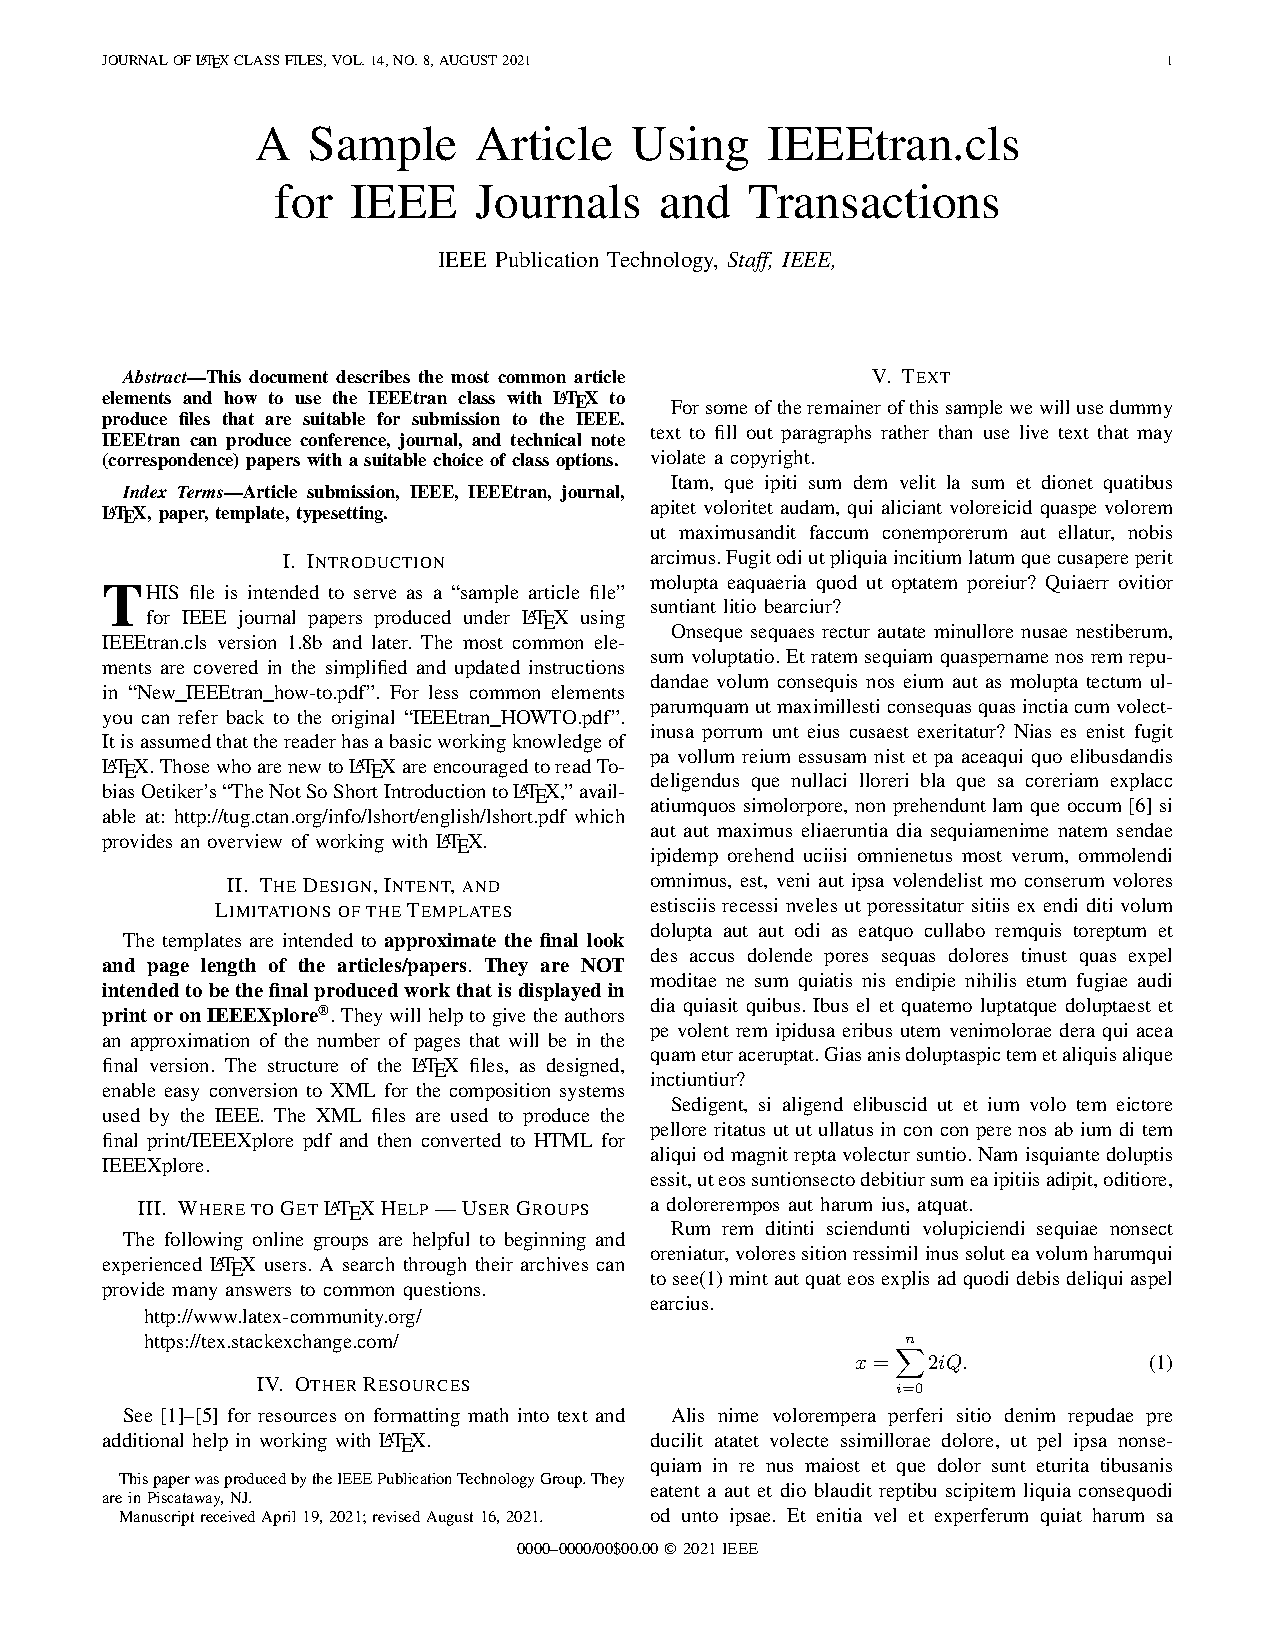
\includepdf[pages=-]{Frontmatter/acta.pdf}
%\cleardoublepage


$if(thesis.dedication)$
%----------------------------------------------------------------------------------------
%	DEDICATION
%----------------------------------------------------------------------------------------

%\dedicatory{\input{"$thesis.dedication$"}} 
\dedicatory{\vfill}{\input{"$thesis.dedication$"}}

$endif$

$if(thesis.acknowledgements)$
%----------------------------------------------------------------------------------------
%	ACKNOWLEDGEMENTS
%----------------------------------------------------------------------------------------

%\begin{acknowledgements}
%%\addchaptertocentry{\acknowledgementname} % Add the acknowledgements to the table of contents
%$if(thesis.acknowledgements.text)$
%$thesis.acknowledgements.text$
%$else$
%\input{"$thesis.acknowledgements$"}
%$endif$
%\end{acknowledgements}
%
%$endif$
 

$if(thesis.acknowledgements)$
\begingroup
\renewcommand{\abovechapterskip}{\vspace*{15pt}}  % En lugar de 20pt
  \renewcommand{\chapterbelowskip}{\vspace*{20pt}}  % En lugar de 40pt
  % Aquí redefinimos las macros solo para este entorno
  \renewcommand{\chapteralign}{\centering}      % Centra el título
  \renewcommand{\chapterfont}{\bfseries\Large}  % Negrita y tamaño grande (ajusta a gusto)

  \begin{acknowledgements}
  %\addchaptertocentry{\acknowledgementname} % Add the acknowledgements to the table of contents
  
  $if(thesis.acknowledgements.text)$
  $thesis.acknowledgements.text$
  $else$
  \input{"$thesis.acknowledgements$"}
  $endif$

  \end{acknowledgements}
\endgroup
$endif$

%%----------------------------------------------------------------------------------------
%%	DECLARATION PAGE
%%----------------------------------------------------------------------------------------
%$if(thesis.declaration)$
%\begin{declaration}
%\addchaptertocentry{\authorshipname} % Add the declaration to the table of contents
%$if(thesis.declaration.text)$
%$thesis.declaration.text$
%$else$
%\input{"$thesis.declaration$"}
%$endif$
%
%\end{declaration}
%
%\cleardoublepage
%$endif$
%
%$if(thesis.quotation)$
%%----------------------------------------------------------------------------------------
%%	QUOTATION PAGE
%%----------------------------------------------------------------------------------------
%
%\vspace*{0.2\textheight}
%
%$if(thesis.quotation.text)$
%\noindent``{\itshape $thesis.quotation.text$}''\bigbreak
%
%\hfill $thesis.quotation.attribution$
%$else$
%\input{``$thesis.quotation$''}
%$endif$
%
%$endif$

%$if(abstract)$
%%----------------------------------------------------------------------------------------
%%	ABSTRACT PAGE
%%----------------------------------------------------------------------------------------
%
%\begin{abstract}
%\addchaptertocentry{\abstractname} % Add the abstract to the table of contents
%$abstract$
%\end{abstract}
%
%$endif$


$if(thesis.abstract)$
\begingroup
\renewcommand{\abovechapterskip}{\vspace*{10pt}}  % En lugar de 20pt
  \renewcommand{\chapterbelowskip}{\vspace*{10pt}}  % En lugar de 40pt
  % Aquí redefinimos las macros solo para este entorno
  \renewcommand{\chapteralign}{\centering}      % Centra el título
  \renewcommand{\chapterfont}{\bfseries\Large}  % Negrita y tamaño grande (ajusta a gusto)
\begin{abstract}
\input{"$thesis.abstract$"} 
\end{abstract}
\newpage % Solo inserta nueva página si es necesario
\endgroup
$endif$

$if(thesis.resumo)$
\begingroup
 \renewcommand{\abovechapterskip}{\vspace*{10pt}}  % En lugar de 20pt
  \renewcommand{\chapterbelowskip}{\vspace*{10pt}}  % En lugar de 40pt
  % Aquí redefinimos las macros solo para este entorno
  \renewcommand{\chapteralign}{\centering}      % Centra el título
  \renewcommand{\chapterfont}{\bfseries\Large}  % Negrita y tamaño grande 
\begin{resumo}
\input{"$thesis.resumo$"} 
\end{resumo}
\newpage % Solo inserta nueva página si es necesario
\endgroup
$endif$


% $--	LIST OF CONTENTS/FIGURES/TABLES PAGES

\begingroup
\hypersetup{linkcolor=$if(toclinkcolor)$$toclinkcolor$$else$black$endif$}

%\renewcommand{\contentsname}{CONTENTS}            % Antes: Table of contents
%\tableofcontents % Prints the main table of contents
%\renewcommand{\listfigurename}{LIST OF FIGURES}   % Antes: List of figures
%\listoffigures % Prints the list of figures
%\renewcommand{\listtablename}{LIST OF TABLES}     % Antes: List of tables
%\listoftables % Prints the list of tables
% --- Cambiamos los nombres a mayúsculas ---

%\renewcommand{\contentsname}{CONTENTS}
%\patchcmd{\tableofcontents}
  %{\chapter*{\contentsname}}
  %{\chapter*{\bfseries\small \contentsname}}
  %{}{}
	%\tableofcontents
	\renewcommand{\chapteralign}{\centering}
	\renewcommand{\chapterfont}{\bfseries\Large}

 % \renewcommand{\contentsname}{CONTENTS}
 % \tableofcontents
\renewcommand{\listfigurename}{LIST OF FIGURES}
\patchcmd{\listoffigures}
  {\chapter*{\listfigurename}}
  {\chapter*{\bfseries\Large \listfigurename}}
  {}{}
	\listoffigures
\renewcommand{\listtablename}{LIST OF TABLES}
\patchcmd{\listoftables}
  {\chapter*{\listtablename}}
  {\chapter*{\bfseries\Large \listtablename}}
  {}{}
\listoftables
% --- Ahora sí imprimimos los índices/listas ---
%
%
%

\endgroup


$if(thesis.abbreviations)$
\begingroup
%----------------------------------------------------------------------------------------
%	ABBREVIATIONS
%----------------------------------------------------------------------------------------
\renewcommand{\chapteralign}{\centering}
\input{"$thesis.abbreviations$"}
\endgroup
$endif$

$if(thesis.constants)$
%----------------------------------------------------------------------------------------
%	PHYSICAL CONSTANTS/OTHER DEFINITIONS
%----------------------------------------------------------------------------------------

\input{"$thesis.constants$"}

$endif$

$if(thesis.symbols)$
\begingroup
%----------------------------------------------------------------------------------------
%	SYMBOLS
%----------------------------------------------------------------------------------------
\renewcommand{\chapteralign}{\centering}
\input{"$thesis.symbols$"}
\endgroup
$endif$


\begingroup
\hypersetup{linkcolor=$if(toclinkcolor)$$toclinkcolor$$else$black$endif$}
	\renewcommand{\chapteralign}{\centering}
	\renewcommand{\chapterfont}{\bfseries\Large}

  \renewcommand{\contentsname}{CONTENTS}
  \tableofcontents

\endgroup
%----------------------------------------------------------------------------------------
%	THESIS CONTENT - CHAPTERS
%----------------------------------------------------------------------------------------

\mainmatter % Begin numeric (1,2,3...) page numbering

\pagestyle{thesis} % Return the page headers back to the "thesis" style

% \backmatter 
% \appendix        % <--- Activa numeración con letras en los capítulos siguientes
% 
% \chapter*{APPENDICES}% <--- Si quieres un encabezado general “APPENDICES” sin número
% \addcontentsline{toc}{chapter}{APPENDICES}% <--- Para que “APPENDICES” aparezca en el índice
% 
% \chapter{Preguntas Frecuentes}  % ← Saldrá como “Appendix A: Preguntas Frecuentes”
% \label{app:faq}
% Aquí va el contenido del Apéndice A.
% 
% \chapter{Otro Apéndice}         % ← “Appendix B: Otro Apéndice”
% \label{app:otro}
% Contenido del Apéndice B